% CVPR 2025 Paper Template; see https://github.com/cvpr-org/author-kit

\documentclass[10pt,twocolumn,letterpaper]{article}

%%%%%%%%% PAPER TYPE  - PLEASE UPDATE FOR FINAL VERSION
\usepackage{cvpr}              % To produce the CAMERA-READY version
% \usepackage[review]{cvpr}      % To produce the REVIEW version
% \usepackage[pagenumbers]{cvpr} % To force page numbers, e.g. for an arXiv version

\usepackage{multirow}
\usepackage[export]{adjustbox}

% Import additional packages in the preamble file, before hyperref
%
% --- inline annotations
%
\newcommand{\red}[1]{{\color{red}#1}}
\newcommand{\todo}[1]{{\color{red}#1}}
\newcommand{\TODO}[1]{\textbf{\color{red}[TODO: #1]}}
% --- disable by uncommenting  
% \renewcommand{\TODO}[1]{}
% \renewcommand{\todo}[1]{#1}



% It is strongly recommended to use hyperref, especially for the review version.
% hyperref with option pagebackref eases the reviewers' job.
% Please disable hyperref *only* if you encounter grave issues, 
% e.g. with the file validation for the camera-ready version.
%
% If you comment hyperref and then uncomment it, you should delete *.aux before re-running LaTeX.
% (Or just hit 'q' on the first LaTeX run, let it finish, and you should be clear).
\definecolor{cvprblue}{rgb}{0.21,0.49,0.74}
\usepackage[pagebackref,breaklinks,colorlinks,allcolors=cvprblue]{hyperref}

%%%%%%%%% PAPER ID  - PLEASE UPDATE
\def\paperID{*****} % *** Enter the Paper ID here
\def\confName{CVPR}
\def\confYear{2025}

%%%%%%%%% TITLE - PLEASE UPDATE
\title{Understanding the Structural information captured by 3D shapes encoders}

%%%%%%%%% AUTHORS - PLEASE UPDATE
\author{Louis Martinez\\
Télécom Paris\\
{\tt\small louis.martinez@telecom-paris.fr}
% For a paper whose authors are all at the same institution,
% omit the following lines up until the closing ``}''.
% Additional authors and addresses can be added with ``\and'',
% just like the second author.
% To save space, use either the email address or home page, not both
}

\begin{document}
\maketitle
\begin{abstract}
Transformers have become the dominant architecture for representation learning across modalities, achieving strong performance in natural language processing and computer vision. This has motivated recent efforts to extend transformers to 3D shape understanding. While these models show promising results, they face two fundamental challenges. First, transformers are notoriously data-hungry, yet even the largest 3D shape datasets remain orders of magnitude smaller than those in text or vision. Second, although transformers perform well on simple benchmarks, they struggle with tasks that require reasoning about complex geometries and topologies. In particular, it is unclear whether pretrained 3D transformer models capture the structural, non-semantic properties of shapes, beyond surface-level geometric or categorical information. In this work, we systematically investigate this question. We demonstrate that current 3D transformers are intrinsically limited in their ability to capture such structural information, and we introduce a new procedure (tbd) that addresses this limitation and improves their capacity to represent challenging 3D shape properties.
\end{abstract}    
\section{Introduction}
\label{sec:intro}

Foundation models for 3D data have recently emerged a promising direction for scaling 3D shapes analysis. Inspired by the success of large language models and images encoders, especially the expressivity of the learned representations, this paradigm has been adapted to 3D shapes, leading to significant improvements in various tasks such as shape classification, segmentation, and generation. These models are pretrained on vast amounts of unlabeled 3D data to learn rich representations that can be further fine-tuned for downstream tasks, enabling better generalization. Although these models can capture semantic and geometric information from 3D shapes quite well, it remains unclear to what extent they also encode non-semantic, structural information, such as the topology. More generally, pretraining procedures for 3D shapes encoders have been directly adapted from the image and text domains, without considering the specific characteristics of 3D data. As a consequence, sate-of-the-art methods have a fairly limited range of validity. For instance, models trained on object centric data can't generalize to larger scenes, while models aimed to process large scenes struggle in capturing fine-grained details. This raises the question of whether these models are truly capable of capturing the unique properties of 3D shapes at different scales, or if they simply learn to mimic the patterns found in the training data. The actual quality of the learned representations remains an open question. In this report, we aim to shed light on these issues by investigating the extent to which 3D shapes encoders capture structural information, and how this impacts their performance across different tasks and scales. We also explore the limitations of current pretraining procedures and propose potential improvements to enhance the robustness and generalization capabilities of 3D shapes encoders. 

The contributions of this report are 3-folds:

\begin{itemize}
    \item We introduce TopoGen, a scalable dataset of 3D shapes with full control over the topology of the generated 3D shapes
    \item We carry out comprehensive experiments to understand and quantify to what extent current state-of-the-art 3D shape encoders capture structural, non-semantic information from 3D shapes.
    \item Guided by the results obtained from our experiments, we propose architectural improvements and pretraining strategies to encourage the presence of such properties.
\end{itemize}

%-------------------------------------------------------------------------
% \subsection{Language}

% All manuscripts must be in English.

% \subsection{Dual submission}

% Please refer to the author guidelines on the \confName\ \confYear\ web page for a
% discussion of the policy on dual submissions.

% \subsection{Paper length}
% Papers, excluding the references section, must be no longer than eight pages in length.
% The references section will not be included in the page count, and there is no limit on the length of the references section.
% For example, a paper of eight pages with two pages of references would have a total length of 10 pages.
% {\bf There will be no extra page charges for \confName\ \confYear.}

% Overlength papers will simply not be reviewed.
% This includes papers where the margins and formatting are deemed to have been significantly altered from those laid down by this style guide.
% Note that this \LaTeX\ guide already sets figure captions and references in a smaller font.
% The reason such papers will not be reviewed is that there is no provision for supervised revisions of manuscripts.
% The reviewing process cannot determine the suitability of the paper for presentation in eight pages if it is reviewed in eleven.

% %-------------------------------------------------------------------------
% \subsection{The ruler}
% The \LaTeX\ style defines a printed ruler which should be present in the version submitted for review.
% The ruler is provided in order that reviewers may comment on particular lines in the paper without circumlocution.
% If you are preparing a document using a non-\LaTeX\ document preparation system, please arrange for an equivalent ruler to appear on the final output pages.
% The presence or absence of the ruler should not change the appearance of any other content on the page.
% The camera-ready copy should not contain a ruler.
% (\LaTeX\ users may use options of \texttt{cvpr.sty} to switch between different versions.)

% Reviewers:
% note that the ruler measurements do not align well with lines in the paper --- this turns out to be very difficult to do well when the paper contains many figures and equations, and, when done, looks ugly.
% Just use fractional references (\eg, this line is $087.5$), although in most cases one would expect that the approximate location will be adequate.


% \subsection{Paper ID}
% Make sure that the Paper ID from the submission system is visible in the version submitted for review (replacing the ``*****'' you see in this document).
% If you are using the \LaTeX\ template, \textbf{make sure to update paper ID in the appropriate place in the tex file}.


% \subsection{Mathematics}

% Please number all of your sections and displayed equations as in these examples:
% \begin{equation}
%   E = m\cdot c^2
%   \label{eq:important}
% \end{equation}
% and
% \begin{equation}
%   v = a\cdot t.
%   \label{eq:also-important}
% \end{equation}
% It is important for readers to be able to refer to any particular equation.
% Just because you did not refer to it in the text does not mean some future reader might not need to refer to it.
% It is cumbersome to have to use circumlocutions like ``the equation second from the top of page 3 column 1''.
% (Note that the ruler will not be present in the final copy, so is not an alternative to equation numbers).
% All authors will benefit from reading Mermin's description of how to write mathematics:
% \url{http://www.pamitc.org/documents/mermin.pdf}.

% \subsection{Blind review}

% Many authors misunderstand the concept of anonymizing for blind review.
% Blind review does not mean that one must remove citations to one's own work---in fact it is often impossible to review a paper unless the previous citations are known and available.

% Blind review means that you do not use the words ``my'' or ``our'' when citing previous work.
% That is all.
% (But see below for tech reports.)

% Saying ``this builds on the work of Lucy Smith [1]'' does not say that you are Lucy Smith;
% it says that you are building on her work.
% If you are Smith and Jones, do not say ``as we show in [7]'', say ``as Smith and Jones show in [7]'' and at the end of the paper, include reference 7 as you would any other cited work.

% An example of a bad paper just asking to be rejected:
% \begin{quote}
% \begin{center}
%     An analysis of the frobnicatable foo filter.
% \end{center}

%    In this paper we present a performance analysis of our previous paper [1], and show it to be inferior to all previously known methods.
%    Why the previous paper was accepted without this analysis is beyond me.

%    [1] Removed for blind review
% \end{quote}


% An example of an acceptable paper:
% \begin{quote}
% \begin{center}
%      An analysis of the frobnicatable foo filter.
% \end{center}

%    In this paper we present a performance analysis of the  paper of Smith \etal [1], and show it to be inferior to all previously known methods.
%    Why the previous paper was accepted without this analysis is beyond me.

%    [1] Smith, L and Jones, C. ``The frobnicatable foo filter, a fundamental contribution to human knowledge''. Nature 381(12), 1-213.
% \end{quote}

% If you are making a submission to another conference at the same time, which covers similar or overlapping material, you may need to refer to that submission in order to explain the differences, just as you would if you had previously published related work.
% In such cases, include the anonymized parallel submission~\cite{Authors14} as supplemental material and cite it as
% \begin{quote}
% [1] Authors. ``The frobnicatable foo filter'', F\&G 2014 Submission ID 324, Supplied as supplemental material {\tt fg324.pdf}.
% \end{quote}

% Finally, you may feel you need to tell the reader that more details can be found elsewhere, and refer them to a technical report.
% For conference submissions, the paper must stand on its own, and not {\em require} the reviewer to go to a tech report for further details.
% Thus, you may say in the body of the paper ``further details may be found in~\cite{Authors14b}''.
% Then submit the tech report as supplemental material.
% Again, you may not assume the reviewers will read this material.

% Sometimes your paper is about a problem which you tested using a tool that is widely known to be restricted to a single institution.
% For example, let's say it's 1969, you have solved a key problem on the Apollo lander, and you believe that the 1970 audience would like to hear about your
% solution.
% The work is a development of your celebrated 1968 paper entitled ``Zero-g frobnication: How being the only people in the world with access to the Apollo lander source code makes us a wow at parties'', by Zeus \etal.

% You can handle this paper like any other.
% Do not write ``We show how to improve our previous work [Anonymous, 1968].
% This time we tested the algorithm on a lunar lander [name of lander removed for blind review]''.
% That would be silly, and would immediately identify the authors.
% Instead write the following:
% \begin{quotation}
% \noindent
%    We describe a system for zero-g frobnication.
%    This system is new because it handles the following cases:
%    A, B.  Previous systems [Zeus et al. 1968] did not  handle case B properly.
%    Ours handles it by including a foo term in the bar integral.

%    ...

%    The proposed system was integrated with the Apollo lunar lander, and went all the way to the moon, don't you know.
%    It displayed the following behaviours, which show how well we solved cases A and B: ...
% \end{quotation}
% As you can see, the above text follows standard scientific convention, reads better than the first version, and does not explicitly name you as the authors.
% A reviewer might think it likely that the new paper was written by Zeus \etal, but cannot make any decision based on that guess.
% He or she would have to be sure that no other authors could have been contracted to solve problem B.
% \medskip

% \noindent
% FAQ\medskip\\
% {\bf Q:} Are acknowledgements OK?\\
% {\bf A:} No.  Leave them for the final copy.\medskip\\
% {\bf Q:} How do I cite my results reported in open challenges?
% {\bf A:} To conform with the double-blind review policy, you can report results of other challenge participants together with your results in your paper.
% For your results, however, you should not identify yourself and should not mention your participation in the challenge.
% Instead present your results referring to the method proposed in your paper and draw conclusions based on the experimental comparison to other results.\medskip\\

% \begin{figure}[t]
%   \centering
%   \fbox{\rule{0pt}{2in} \rule{0.9\linewidth}{0pt}}
%    %\includegraphics[width=0.8\linewidth]{egfigure.eps}

%    \caption{Example of caption.
%    It is set in Roman so that mathematics (always set in Roman: $B \sin A = A \sin B$) may be included without an ugly clash.}
%    \label{fig:onecol}
% \end{figure}

% \subsection{Miscellaneous}

% \noindent
% Compare the following:\\
% \begin{tabular}{ll}
%  \verb'$conf_a$' &  $conf_a$ \\
%  \verb'$\mathit{conf}_a$' & $\mathit{conf}_a$
% \end{tabular}\\
% See The \TeX book, p165.

% The space after \eg, meaning ``for example'', should not be a sentence-ending space.
% So \eg is correct, {\em e.g.} is not.
% The provided \verb'\eg' macro takes care of this.

% When citing a multi-author paper, you may save space by using ``et alia'', shortened to ``\etal'' (not ``{\em et.\ al.}'' as ``{\em et}'' is a complete word).
% If you use the \verb'\etal' macro provided, then you need not worry about double periods when used at the end of a sentence as in Alpher \etal.
% However, use it only when there are three or more authors.
% Thus, the following is correct:
%    ``Frobnication has been trendy lately.
%    It was introduced by Alpher~\cite{Alpher02}, and subsequently developed by
%    Alpher and Fotheringham-Smythe~\cite{Alpher03}, and Alpher \etal~\cite{Alpher04}.''

% This is incorrect: ``... subsequently developed by Alpher \etal~\cite{Alpher03} ...'' because reference~\cite{Alpher03} has just two authors.

% \begin{figure*}
%   \centering
%   \begin{subfigure}{0.68\linewidth}
%     \fbox{\rule{0pt}{2in} \rule{.9\linewidth}{0pt}}
%     \caption{An example of a subfigure.}
%     \label{fig:short-a}
%   \end{subfigure}
%   \hfill
%   \begin{subfigure}{0.28\linewidth}
%     \fbox{\rule{0pt}{2in} \rule{.9\linewidth}{0pt}}
%     \caption{Another example of a subfigure.}
%     \label{fig:short-b}
%   \end{subfigure}
%   \caption{Example of a short caption, which should be centered.}
%   \label{fig:short}
% \end{figure*}

\section{TopoGen Dataset}
\label{sec:topogen}

Assessing how models understand the topology of 3D shapes, in particular through probing, requires data labeled with topological information and control over the distribution of the labels. However such dataset, specifically designed with a focus on the structure and not the semantics, hasn't been developed yet. Hence we introduce TopoGen, a scalable dataset of 3D synthetic shapes with accurate and well balanced topological labels. The samples in this dataset are labeled by number of connected components and genus.

\subsection{Existing datasets}
\label{ssec:existing_datasets}

When speaking about structural understanding, representations such as the ones present in the MANTRA \cite{mantra} dataset are a natural choice. The MANTRA dataset (Manifold Triangulation Assemblage) by Ballester et al. consists purely of combinatorial triangulation of 2- and 3-dimensional manifolds: i.e., its samples only include connectivity information (abstract simplicial complexes), without any geometric embedding in $\mathbb{R}^3$, making it agnostic to geometric realization. This makes MANTRA a particularly meaningful benchmark when assessing whether graph-based and simplicial complex-based models capture higher-order structures (essentially Betti numbers $\beta_0, \beta_1, \beta_2$ and $\beta_3$). However, in this work we focus on evaluating models that rely on geometric 3D representations such as meshes, point clouds, or implicit fields (e.g., Signed Distance Functions (SDFs)) (i.e., data embedded in $\mathbb{R}^3$. Therefore, MANTRA falls outside the scope of the tasks considered in this report.


Only a few large datasets have some considerations about structural information carried by meshes (commonly the number of connected components and the genus). Notably, the Thingi10K and ABC datasets, which are composed with various CAD models and artistic meshes come with such annotations. However, they turn out to be inaccurate for three reasons. 
\begin{enumerate}
  \item \textbf{Discrepancy between actual and effective number of components.} In artistic 3D modeling, a complex shape is often constructed from many mesh objects that represent fine details (buttons, ornaments, small extrusions, etc.). As a result, the true number of connected components in the mesh (counting every individual object used in the construction) can be much larger than the effective number of connected components, which corresponds to the main perceived object as a whole. (*+fig*). The same issue holds with complex CAD models.
  \item \textbf{Imbalanced annotations.} While both Thingi10K and ABC exhibit a wide range of genus values (Figure \ref{fig:thingi-genus} ADD FOR ABC), the distribution is highly imbalanced. For evaluation tasks such as probing, balanced annotations are crucial, yet in this dataset the vast majority of samples have very low genus (typically between 0 and 2), whereas high-genus shapes are severely underrepresented.
  \item \textbf{Structural artifacts.} Most meshes in these datasets are not suitable out-of-the-box for topological labelling. Many of them are non-manifold or contain self-intersecting faces. This raises two main issues. First, it makes topological analysis unreliable: for example, the Euler Characteristic (Equation \ref{eq:euler}) cannot be applied to non-manifold meshes.
\end{enumerate}
\begin{equation}
  \chi = V - E + F = 2 - 2g - b + c
  \label{eq:euler}
\end{equation}
Where $V, E, F$ are the number of vertices, edges and faces respectively, $g$ is the genus, $b$ the number of boundary components and $c$ the number of connected components.

\begin{figure}[t]
  \centering
  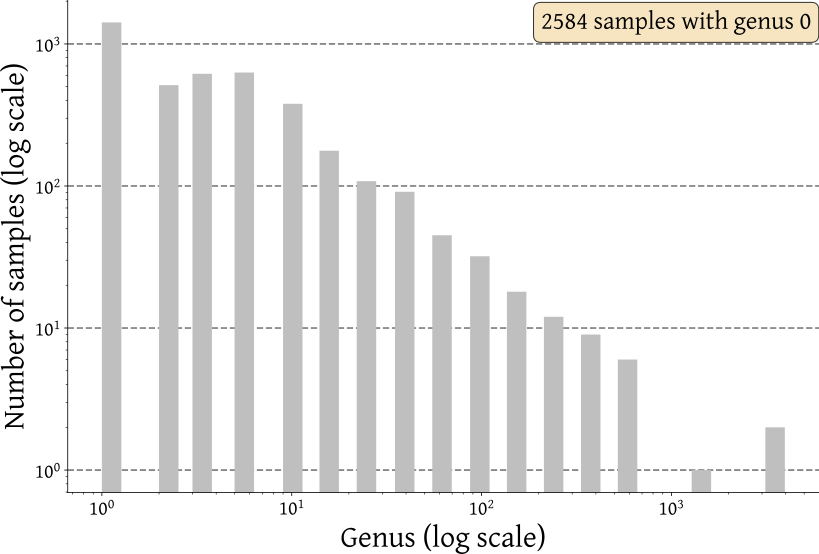
\includegraphics[width=\linewidth]{figs/topogen/thingi_genus_hist.pdf}
   \caption{\textbf{Genus distribution of Thingi10K.} Both axes are plotted in log scale. The genus was estimated from the Euler characteristic, provided as metadata with the dataset; however, 2,651 samples do not fulfill the requirements to directly compute the genus from the Euler characteristic (see \ref{eq:euler}). They are therefore not taken into account here. The histogram shows that a large fraction of the dataset (over 3,000 samples out of 7,344) has genera of 0 or 1, indicating that higher-genus components are significantly underrepresented, which may limit accurate classification and probing analyses for those cases.}
   \label{fig:thingi-genus}
\end{figure}


Second, self-intersections may introduce undesired topological structures, leading to inaccurate labels. To overcome these issues, remeshing procedures such as Manifold \cite{manifold} and ManifoldPlus \cite{manifoldplus} were proposed, transforming arbitrary meshes into manifold and watertight representations. While Manifold provides robustness, it often over smooths the input geometry, reducing fine details. ManifoldPlus improves accuracy but introduces artifacts (see Fig...) (*+example with flower pot*) in challenging cases, leading to inconsistencies in the resulting topology. More recent approaches rely on intermediate representations such as signed or unsigned distance fields. Methods like Dual Octree Graph Networks (DOGN) \cite{dogn}, and the remeshing procedure in CLAY \cite{clay} achieve more stable and reliable results, but at the cost of significantly higher computational complexity. Finally, some shapes in Thingi10K and ABC also exhibit highly uneven geometric complexity, which can negatively impact model evaluation. To ensure that results primarily reflect the topology of the shapes, a certain level of uniformity in geometric complexity across the dataset is necessary. However, quantifying geometric difficulty is challenging, as no straightforward metric exists to assess it. Moreover, since the shapes were not generated under a controlled process, it is not possible to design a general heuristic to filter out geometrically challenging samples consistently.


% Finally, the EuLearn dataset (Figure \ref{fig:eulearn-samples}), intended to supervise models on inferring the genus from point clouds, offers interesting perspectives to train on synthetic data. The dataset is generated from Fourier curves with additional procedures to create knots, which in turn produce surfaces of different genera and some topological diversity. Despite its scalability in terms of the number of samples, EuLearn only covers genera between 0 and 10. Moreover, the generation rules lead to very limited variation within each genus: samples of the same class tend to look too similar, which results in strong overfitting. @fig:eulearn_umap_aug and @tab:eulearn_overfit highlight this issue at the transformer features level while @fig:eulearn_samples and @fig:eulearn_acc_angle confirm this issue at the sample level. In particular, @fig:eulearn_acc_angle exhibits a strong correlation between shapes genera and their canonical orientation. Indeed, a simple nearest neighbors classifier with Chamfer distance achieves perfect accuracy on the test set if it's fit on the training set as is. Beyond this rotation-genus correlation, @fig:eulearn_face_to_vertex_ratio further shows that the geometric complexity (as measured by the face-to-vertex ratio) is strongly correlated with the genus. This correlation makes it difficult to disentangle whether classification performance is driven by topological information or by correlated geometric cues. Overall, these limitations make EuLearn unsuitable for robustly probing structural understanding in 3D shape encoders.

\begin{figure}[t]
  \centering
  \includegraphics[width=\linewidth]{figs/topogen/eulearn_samples.pdf}
   \caption{\textbf{Samples from the EuLearn dataset across different genera.} As the genus increases, shapes become geometrically more complex. This trend highlights a confounding factor in the dataset: geometric complexity grows together with genus. As a result, classification performance may be driven not only by topological information but also by correlated geometric cues.}
   \label{fig:eulearn-samples}
\end{figure}

% All text must be in a two-column format.
% The total allowable size of the text area is $6\frac78$ inches (17.46 cm) wide by $8\frac78$ inches (22.54 cm) high.
% Columns are to be $3\frac14$ inches (8.25 cm) wide, with a $\frac{5}{16}$ inch (0.8 cm) space between them.
% The main title (on the first page) should begin 1 inch (2.54 cm) from the top edge of the page.
% The second and following pages should begin 1 inch (2.54 cm) from the top edge.
% On all pages, the bottom margin should be $1\frac{1}{8}$ inches (2.86 cm) from the bottom edge of the page for $8.5 \times 11$-inch paper;
% for A4 paper, approximately $1\frac{5}{8}$ inches (4.13 cm) from the bottom edge of the
% page.

% %-------------------------------------------------------------------------
% \subsection{Margins and page numbering}

% All printed material, including text, illustrations, and charts, must be kept
% within a print area $6\frac{7}{8}$ inches (17.46 cm) wide by $8\frac{7}{8}$ inches (22.54 cm)
% high.
% %
% Page numbers should be in the footer, centered and $\frac{3}{4}$ inches from the bottom of the page.
% The review version should have page numbers, yet the final version submitted as camera ready should not show any page numbers.
% The \LaTeX\ template takes care of this when used properly.



% %-------------------------------------------------------------------------
% \subsection{Type style and fonts}

% Wherever Times is specified, Times Roman may also be used.
% If neither is available on your word processor, please use the font closest in
% appearance to Times to which you have access.

% MAIN TITLE.
% Center the title $1\frac{3}{8}$ inches (3.49 cm) from the top edge of the first page.
% The title should be in Times 14-point, boldface type.
% Capitalize the first letter of nouns, pronouns, verbs, adjectives, and adverbs;
% do not capitalize articles, coordinate conjunctions, or prepositions (unless the title begins with such a word).
% Leave two blank lines after the title.

% AUTHOR NAME(s) and AFFILIATION(s) are to be centered beneath the title
% and printed in Times 12-point, non-boldface type.
% This information is to be followed by two blank lines.

% The ABSTRACT and MAIN TEXT are to be in a two-column format.

% MAIN TEXT.
% Type main text in 10-point Times, single-spaced.
% Do NOT use double-spacing.
% All paragraphs should be indented 1 pica (approx.~$\frac{1}{6}$ inch or 0.422 cm).
% Make sure your text is fully justified---that is, flush left and flush right.
% Please do not place any additional blank lines between paragraphs.

% Figure and table captions should be 9-point Roman type as in \cref{fig:onecol,fig:short}.
% Short captions should be centred.

% \noindent Callouts should be 9-point Helvetica, non-boldface type.
% Initially capitalize only the first word of section titles and first-, second-, and third-order headings.

% FIRST-ORDER HEADINGS.
% (For example, {\large \bf 1. Introduction}) should be Times 12-point boldface, initially capitalized, flush left, with one blank line before, and one blank line after.

% SECOND-ORDER HEADINGS.
% (For example, { \bf 1.1. Database elements}) should be Times 11-point boldface, initially capitalized, flush left, with one blank line before, and one after.
% If you require a third-order heading (we discourage it), use 10-point Times, boldface, initially capitalized, flush left, preceded by one blank line, followed by a period and your text on the same line.

% %-------------------------------------------------------------------------
% \subsection{Footnotes}

% Please use footnotes\footnote{This is what a footnote looks like.
% It often distracts the reader from the main flow of the argument.} sparingly.
% Indeed, try to avoid footnotes altogether and include necessary peripheral observations in the text (within parentheses, if you prefer, as in this sentence).
% If you wish to use a footnote, place it at the bottom of the column on the page on which it is referenced.
% Use Times 8-point type, single-spaced.


% %-------------------------------------------------------------------------
% \subsection{Cross-references}

% For the benefit of author(s) and readers, please use the
% {\small\begin{verbatim}
%   \cref{...}
% \end{verbatim}}  command for cross-referencing to figures, tables, equations, or sections.
% This will automatically insert the appropriate label alongside the cross-reference as in this example:
% \begin{quotation}
%   To see how our method outperforms previous work, please see \cref{fig:onecol} and \cref{tab:example}.
%   It is also possible to refer to multiple targets as once, \eg~to \cref{fig:onecol,fig:short-a}.
%   You may also return to \cref{sec:formatting} or look at \cref{eq:also-important}.
% \end{quotation}
% If you do not wish to abbreviate the label, for example at the beginning of the sentence, you can use the
% {\small\begin{verbatim}
%   \Cref{...}
% \end{verbatim}}
% command. Here is an example:
% \begin{quotation}
%   \Cref{fig:onecol} is also quite important.
% \end{quotation}

% %-------------------------------------------------------------------------
% \subsection{References}

% List and number all bibliographical references in 9-point Times, single-spaced, at the end of your paper.
% When referenced in the text, enclose the citation number in square brackets, for
% example~\cite{Authors14}.
% Where appropriate, include page numbers and the name(s) of editors of referenced books.
% When you cite multiple papers at once, please make sure that you cite them in numerical order like this \cite{Alpher02,Alpher03,Alpher05,Authors14b,Authors14}.
% If you use the template as advised, this will be taken care of automatically.

% \begin{table}
%   \centering
%   \begin{tabular}{@{}lc@{}}
%     \toprule
%     Method & Frobnability \\
%     \midrule
%     Theirs & Frumpy \\
%     Yours & Frobbly \\
%     Ours & Makes one's heart Frob\\
%     \bottomrule
%   \end{tabular}
%   \caption{Results.   Ours is better.}
%   \label{tab:example}
% \end{table}

% %-------------------------------------------------------------------------
% \subsection{Illustrations, graphs, and photographs}

% All graphics should be centered.
% In \LaTeX, avoid using the \texttt{center} environment for this purpose, as this adds potentially unwanted whitespace.
% Instead use
% {\small\begin{verbatim}
%   \centering
% \end{verbatim}}
% at the beginning of your figure.
% Please ensure that any point you wish to make is resolvable in a printed copy of the paper.
% Resize fonts in figures to match the font in the body text, and choose line widths that render effectively in print.
% Readers (and reviewers), even of an electronic copy, may choose to print your paper in order to read it.
% You cannot insist that they do otherwise, and therefore must not assume that they can zoom in to see tiny details on a graphic.

% When placing figures in \LaTeX, it's almost always best to use \verb+\includegraphics+, and to specify the figure width as a multiple of the line width as in the example below
% {\small\begin{verbatim}
%    \usepackage{graphicx} ...
%    \includegraphics[width=0.8\linewidth]
%                    {myfile.pdf}
% \end{verbatim}
% }


% %-------------------------------------------------------------------------
% \subsection{Color}

% Please refer to the author guidelines on the \confName\ \confYear\ web page for a discussion of the use of color in your document.

% If you use color in your plots, please keep in mind that a significant subset of reviewers and readers may have a color vision deficiency; red-green blindness is the most frequent kind.
% Hence avoid relying only on color as the discriminative feature in plots (such as red \vs green lines), but add a second discriminative feature to ease disambiguation.
% \section{Final copy}

% You must include your signed IEEE copyright release form when you submit your finished paper.
% We MUST have this form before your paper can be published in the proceedings.

% Please direct any questions to the production editor in charge of these proceedings at the IEEE Computer Society Press:
% \url{https://www.computer.org/about/contact}.
\clearpage
\setcounter{page}{1}
\maketitlesupplementary


\section{Rationale}
\label{sec:rationale}
% 
Having the supplementary compiled together with the main paper means that:
% 
\begin{itemize}
\item The supplementary can back-reference sections of the main paper, for example, we can refer to \cref{sec:intro};
\item The main paper can forward reference sub-sections within the supplementary explicitly (e.g. referring to a particular experiment); 
\item When submitted to arXiv, the supplementary will already included at the end of the paper.
\end{itemize}
% 
To split the supplementary pages from the main paper, you can use \href{https://support.apple.com/en-ca/guide/preview/prvw11793/mac#:~:text=Delete%20a%20page%20from%20a,or%20choose%20Edit%20%3E%20Delete).}{Preview (on macOS)}, \href{https://www.adobe.com/acrobat/how-to/delete-pages-from-pdf.html#:~:text=Choose%20%E2%80%9CTools%E2%80%9D%20%3E%20%E2%80%9COrganize,or%20pages%20from%20the%20file.}{Adobe Acrobat} (on all OSs), as well as \href{https://superuser.com/questions/517986/is-it-possible-to-delete-some-pages-of-a-pdf-document}{command line tools}.
{
    \small
    \bibliographystyle{ieeenat_fullname}
    \bibliography{main}
}

% WARNING: do not forget to delete the supplementary pages from your submission 
% \clearpage
\setcounter{page}{1}
\maketitlesupplementary


\section{Rationale}
\label{sec:rationale}
% 
Having the supplementary compiled together with the main paper means that:
% 
\begin{itemize}
\item The supplementary can back-reference sections of the main paper, for example, we can refer to \cref{sec:intro};
\item The main paper can forward reference sub-sections within the supplementary explicitly (e.g. referring to a particular experiment); 
\item When submitted to arXiv, the supplementary will already included at the end of the paper.
\end{itemize}
% 
To split the supplementary pages from the main paper, you can use \href{https://support.apple.com/en-ca/guide/preview/prvw11793/mac#:~:text=Delete%20a%20page%20from%20a,or%20choose%20Edit%20%3E%20Delete).}{Preview (on macOS)}, \href{https://www.adobe.com/acrobat/how-to/delete-pages-from-pdf.html#:~:text=Choose%20%E2%80%9CTools%E2%80%9D%20%3E%20%E2%80%9COrganize,or%20pages%20from%20the%20file.}{Adobe Acrobat} (on all OSs), as well as \href{https://superuser.com/questions/517986/is-it-possible-to-delete-some-pages-of-a-pdf-document}{command line tools}.

\end{document}
